\chapter{Daten und Messungen}
\label{chap:dataandmeasure}

%%%%%%%%%%%%%%%%%%%%%%%%%%%%%%%%%%%%%%%%%%%%%%%%%%%%%%%%%%%%
\section{Mobile iBeacons}
\label{sec:dataandmeasurement:mobilebeacon}
%%%%%%%%%%%%%%%%%%%%%%%%%%%%%%%%%%%%%%%%%%%%%%%%%%%%%%%%%%%%
Die mobilen iBeacon verzichten, wie der Name schon andeutet, auf eine feste Stromquelle und werden ausschließlich mit Batterien betrieben.
Zum Einsatz kommen dabei die sogenannten Knopfzellen, welche mit einer Spannung von 3,0 Volt operieren.
Da Bluetooth Low Energy extrem energiesparend arbeitet, geben die Hersteller der Beacons, die Akkulaufzeit mit bis zu zwei Jahren, ohne einen Batteriewechsel an. Diese Laufzeit hängt jedoch auch stark von der gewählten Signalstärke und dem gewählten Sendeintervall zusammen, welche die Laufzeit sehr stark beeinflussen können.

Bisher gibt es wenige Hersteller dieser iBeacons und der Großteil der Produkte befindet sich momentan noch in der Entwicklungsphase. Die genutzten iBeacons von \emph{estimote} und \emph{kontakt.io} sind ebenfalls noch in der Entwicklungsphase und hauptsächlich als Testgeräte für Entwickler ausgelegt. Dabei bleibt jedoch unklar in wie weit sich das fertige Produkt in den technischen Spezifikationen von den aktuellen Prototypen unterscheiden wird.

%%%%%%%%%%%%%%%%%%%%%%%%%%%%%%%%%%%%%%%%%%%%%%%%%%%%%%%%%%%%
\subsection{estimote Beacon}
\label{sec:dataandmeasurement:mobilebeacon:estimote}
%%%%%%%%%%%%%%%%%%%%%%%%%%%%%%%%%%%%%%%%%%%%%%%%%%%%%%%%%%%%
Die Firma \emph{estimote} mit Sitz in Polen, war ein der ersten, die ein funktionstüchtiges iBeacon vorgestellt haben und es in einem \emph{Developer Preview Kit} zum Verkauf anbieten.
Dieses Kit beinhaltet drei verschiedenfarbige Beacons, welche mit einer wiederverwendbaren Klebeschicht an der Unterseite ausgestattet sind. Dies erlaubt das beliebige Anbringen und Abziehen der Beacons auf allen glatten Oberflächen.
\begin{figure}[htb!]
		\centering
	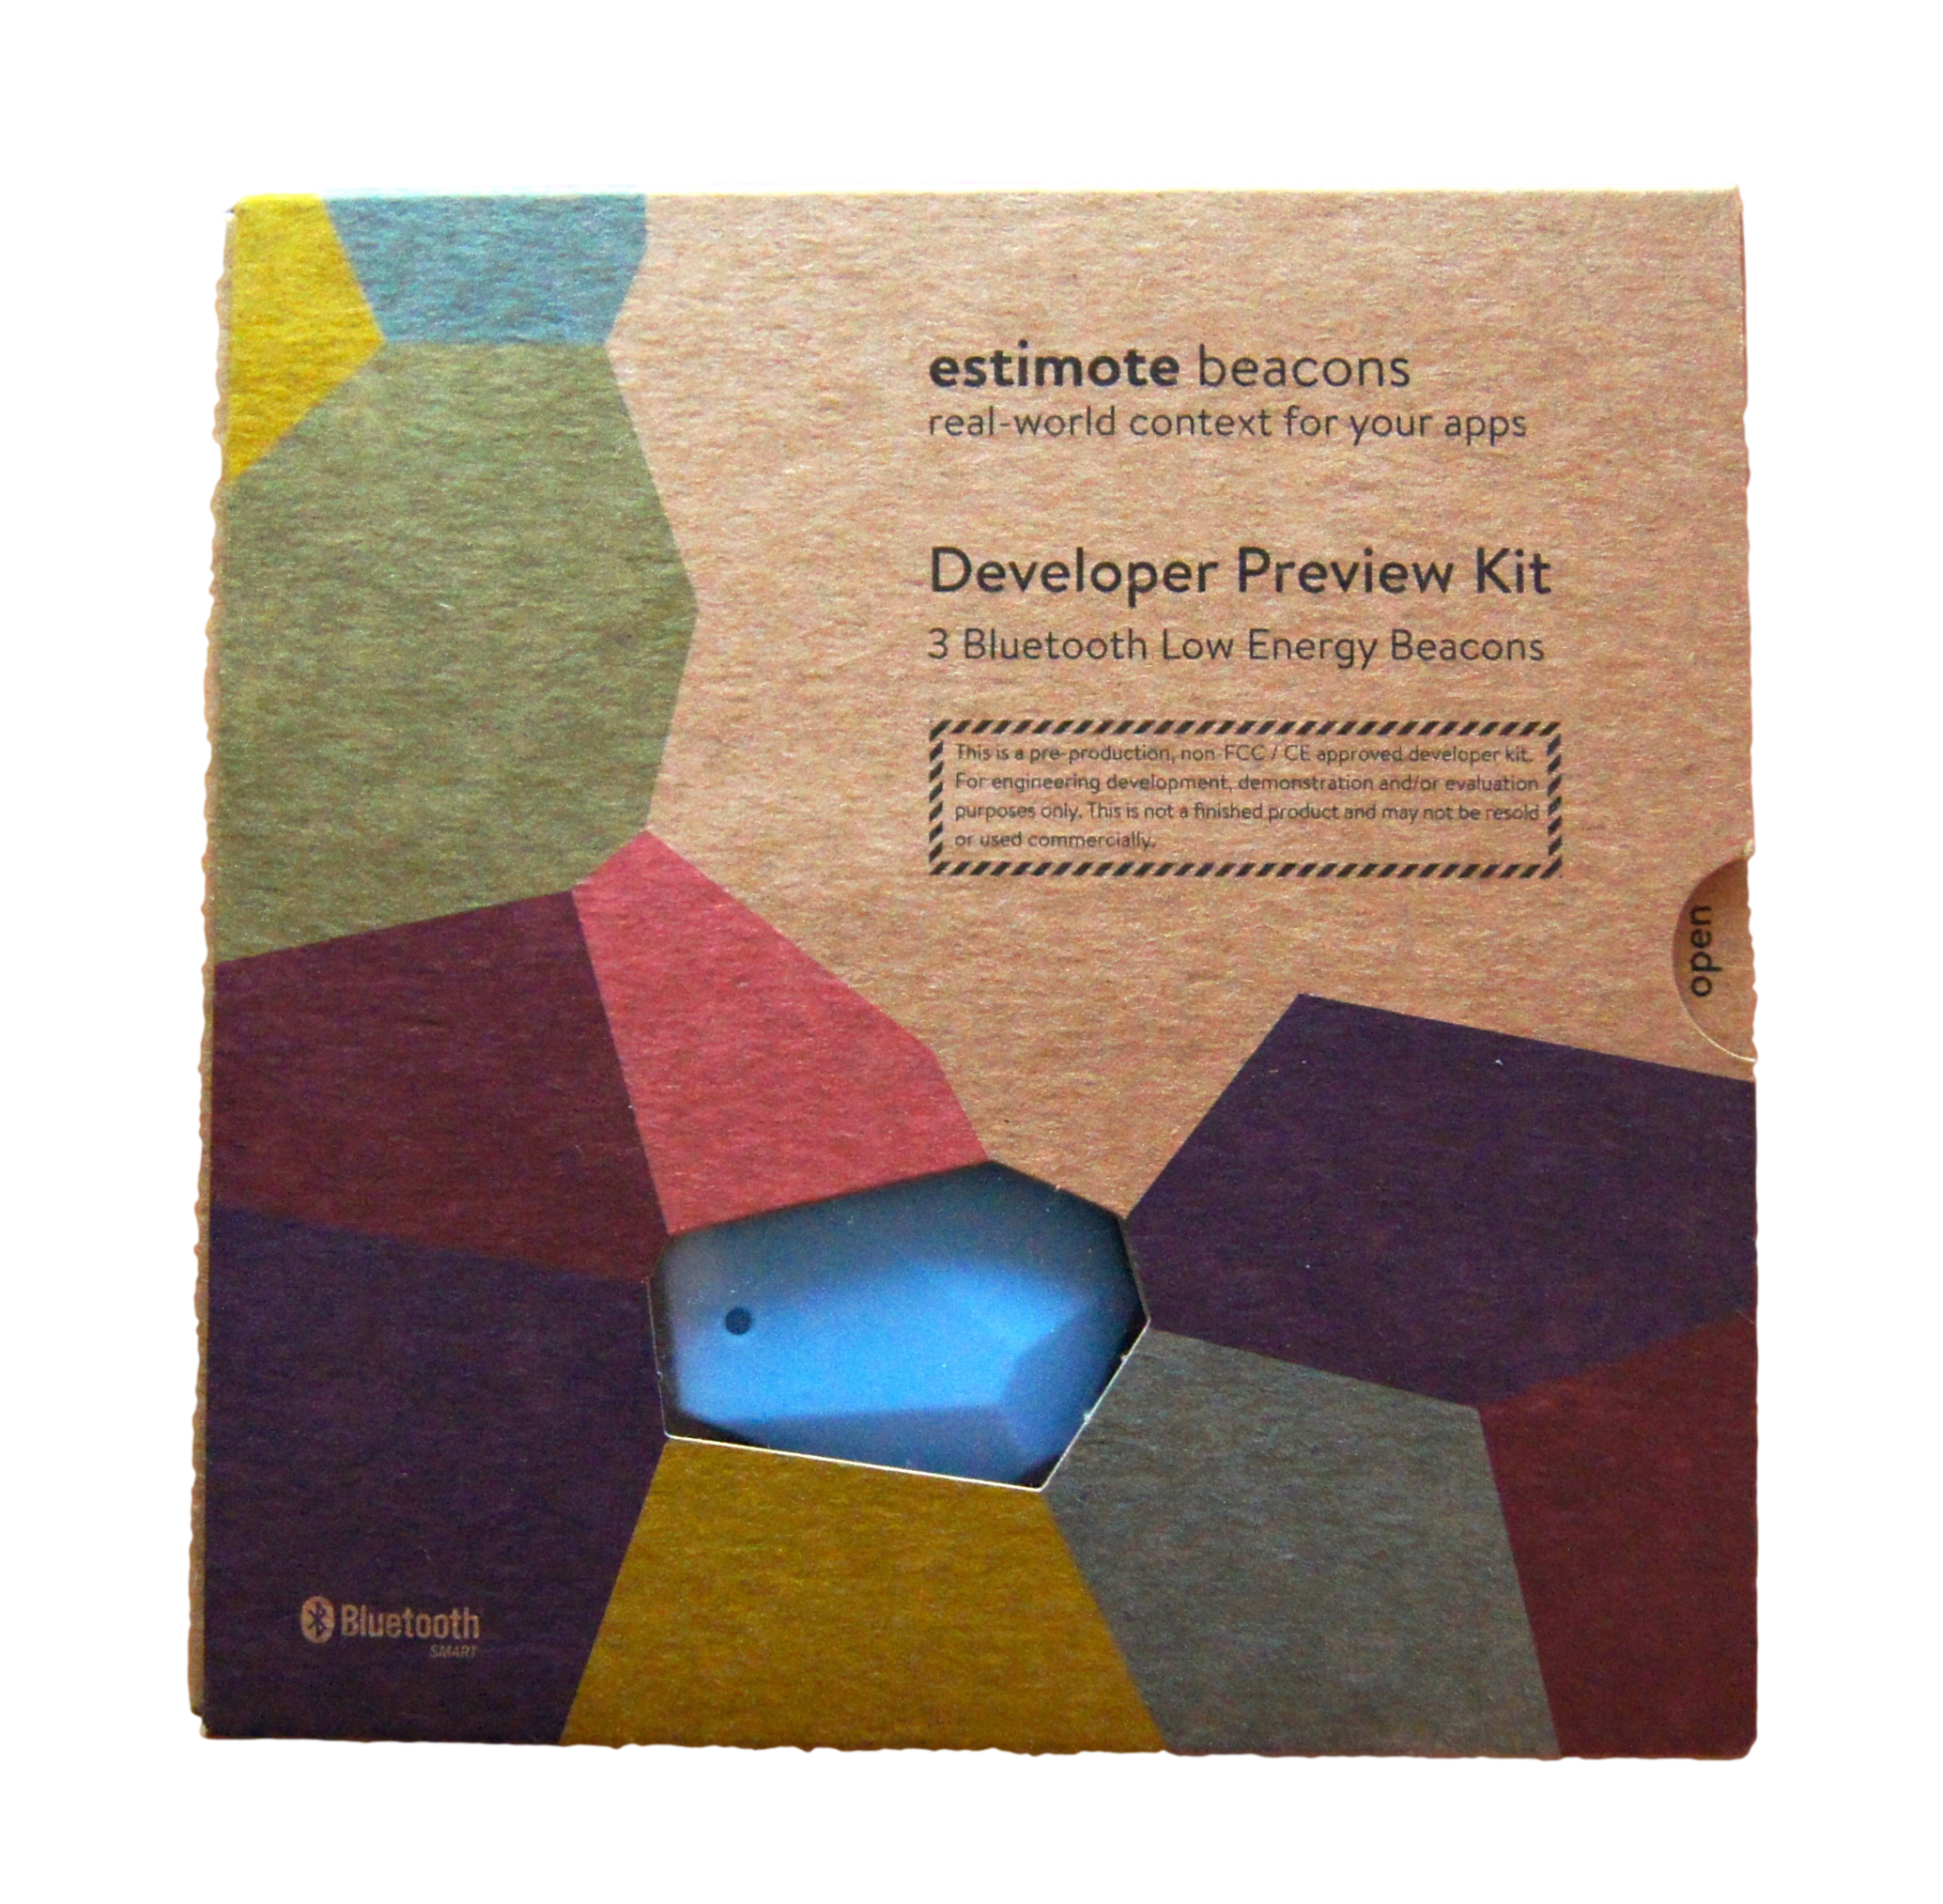
\includegraphics[scale=0.1]{estimote-developer-kit}
	\caption{Das Developer-Kit von estimote}
	\label{estimote-developer-kit}
\end{figure}

Im inneren des Beacons befindet sich ein Bluetooth Chipsatz von Nordic Semiconductor, welcher auf einem 32-bit ARM Prozessor beruht und mit einem 2,4Ghz Bluetooth Low Energy Modul arbeitet. Dabei verfügt der über 256 KB Flash-Speicher für Speicherung der Beacon-Konfiguration.
Speziell in den estimote-Beacon wurde dazu noch ein Temperatursensor eingebaut, welcher allerdings momentan noch nicht angesprochen werden kann.

Des Weiteren stellt estimote noch ein SDK für Android und iOS zur Verfügung, welches in Fall des iOS-SDK auf der iBeacons-API basiert, jedoch speziell auf die estimote-Beacons abgestimmt ist. 
Dabei bietet es neben den Funktionen der iBeacon-API noch die Funktionalität, sich mit den estimote Beacons zu verbinden und diese zu programmieren. So erlaubt es zum Beispiel die Signalstärke, das Sendeintervall und die Major-Minor-Informationen zu verändern oder die Firmware der Beacons zu aktualisieren.

Da das SDK, bis auf die Programmierung der Beacons, keine Vorteile gegenüber dem Core Location-Framework mit der iBeacons-API bietet, wurde jedoch auf die Verwendung verzichtet.

%%%%%%%%%%%%%%%%%%%%%%%%%%%%%%%%%%%%%%%%%%%%%%%%%%%%%%%%%%%%
\subsection{kontakt.io Beacon}
\label{sec:dataandmeasurement:mobilebeacon:kontaktio}
%%%%%%%%%%%%%%%%%%%%%%%%%%%%%%%%%%%%%%%%%%%%%%%%%%%%%%%%%%%%
Ein weiteres Unternehmen, welches sich eine eigene iBeacons-Lösung anbietet ist \emph{kontakt.io}. Auch hier ist noch kein finales Produkt erhältlich, sondern nur ein \emph{Dev Kit}, welches zehn Beacons enthält. 
Die Beacons sind relativ schlicht gehalten und das Innere ist sehr einfach zugänglich, sodass ein Batteriewechsel ohne Umstände möglich ist.


\begin{figure}[htb!]
		\centering
	\includegraphics[scale=0.1]{kontakt-beacon-outside}
	\caption{Kontakt.io Beacon}
	\label{kontakt-beacon-outside}
\end{figure}

Die Beacons von \emph{kontakt.io} basieren dabei auf dem BLE113 Chipsatz von \emph{bluegiga}, welcher über 256 KB Flash-Speicher verfügt und einen 8051 Mikrocontroller von Intel nutzt.


Auch kontakt.io bietet ein eigenes SDK an, welches im Gegensatz zu dem SDK von \emph{estimote} nicht nativ für die einzelnen Plattformen entworfen wurde, sondern online über eine REST-Schnittstelle arbeitet.
Dabei stellt \emph{kontakt.io} ein Webpanel zur Verfügung, in welchem man die einzelnen Beacons mit ihrem UUID, Major und Minor-Wert registriert und jedem den jeweiligen Ort beziehungsweise die Funktion zuweisen kann. 
Auch auf die Verwendung dieses SDK wurde verzichtet.


%%%%%%%%%%%%%%%%%%%%%%%%%%%%%%%%%%%%%%%%%%%%%%%%%%%%%%%%%%%%
\section{Stationäre iBeacons}
\label{sec:dataandmeasurement:stationarybeacon}
%%%%%%%%%%%%%%%%%%%%%%%%%%%%%%%%%%%%%%%%%%%%%%%%%%%%%%%%%%%%
Neben den mobilen iBeacons, welche mittels Batterien funktionieren, gibt es auch stationäre iBeacons, welche auf eine stetige Anbindung an das Stromnetz angewiesen sind.
Dabei gibt es verschiedene Ansätze.
Zum einen bieten zum Beispiel \emph{PayPal} und \emph{Radius Networks} einen Ansatz, bei dem die komplette Technik in einen USB-Stick integriert wird und dann über ein Standart USB-Netzteil an jeder Steckdose betrieben werden kann. Die verwendete Technik dieser Beacons entspricht denen der batteriebetriebenen Beacons.

Eine andere Lösung ist die Nutzung eines Bluetooth 4.0-kompatiblen USB-Dongles an einem Computer. Dieser kann mit entsprechender Software zu einem iBeacon umfunktioniert werden.

%%%%%%%%%%%%%%%%%%%%%%%%%%%%%%%%%%%%%%%%%%%%%%%%%%%%%%%%%%%%
\subsection{Raspberry Pi als iBeacon}
\label{sec:dataandmeasurement:stationarybeacon:raspberrypi}
%%%%%%%%%%%%%%%%%%%%%%%%%%%%%%%%%%%%%%%%%%%%%%%%%%%%%%%%%%%%
Der Raspberry Pi ist ein Mini-Computer, welcher auf einem ARM-Prozessor basiert und als günstiger Computer für Programmiereinsteiger konzipiert wurde. Der kleine Computer ermöglicht aber auch andere Einsatzgebiete, zum Beispiel als Beacon.

Um den Raspberry Pi zu einem Beacon umzufunktionieren wurde eine Linux-Distribution auf dem Gerät installiert und ein Bluetooth-Dongle über USB angeschlossen. Dabei kam ein Modul von \emph{Plugable Technologies} zum Einsatz, welches spezielle Bluetooth 4.0 Unterstützung bietet.
Für die Umfunktionierung zum iBeacon wurde die Bluetooth-Software \emph{blueZ} eingesetzt, welche es erlaubt das Bluetooth-Modul anzusprechen und spezifische Nachrichten über Bluetooth zu schicken.
Diese Möglichkeit wurde von der Firma Radius Network vorgestellt, welche auch ein ausführliches Tutorial für die Nutzung des Raspberry Pi als iBeacon auf ihrer Webseite anbieten (\citet{radiusraspberry}), welches von mir genutzt wurde, um den Raspberry Pi zu konfigurieren.



%%%%%%%%%%%%%%%%%%%%%%%%%%%%%%%%%%%%%%%%%%%%%%%%%%%%%%%%%%%%
\section{Außenmessungen}
\label{sec:dataandmeasurement:outdoormeasure}
%%%%%%%%%%%%%%%%%%%%%%%%%%%%%%%%%%%%%%%%%%%%%%%%%%%%%%%%%%%%

%%%%%%%%%%%%%%%%%%%%%%%%%%%%%%%%%%%%%%%%%%%%%%%%%%%%%%%%%%%%
\section{Innenraummessungen}
\label{sec:dataandmeasurement:indoormeasure}
%%%%%%%%%%%%%%%%%%%%%%%%%%%%%%%%%%%%%%%%%%%%%%%%%%%%%%%%%%%%
Um die Leistungsfähigkeit und das Verhalten der Beacons in Innenräume zu testen und darzustellen, wurden verschiedene Messungen durchgeführt. Dazu wurden zum einen die mobilen Beacons verwendet und zum anderen der Raspberry Pi, als stationäres Beacon.
Die Messungen wurden dabei sowohl mit dem iPhone 5 als auch mit dem iPhone 4s durchführt, um auch hier die Unterschiede zwischen den einzelnen Modellen zu erfassen.


Zuerst wurden die Messungen mit den mobilen Beacons, hier die \emph{kontakt.io}-Beacons, durchgeführt.
Diese wurden in einem leeren, nur an den Wänden bestellten, Raum durchgeführt, wobei immer freie Sicht zwischen den Beacons und den Empfangsgeräten bestand. Für jede Entfernung wurden dabei 100 Stichproben genommen, jeweils eine pro Sekunde.
%%%%%%%%%%%%%%%%%%%%%%%%%%%%%%%%%%%%%%%%%%%%%%%%%%%%%%%%%%%%
% figure of signal strnegth
%%%%%%%%%%%%%%%%%%%%%%%%%%%%%%%%%%%%%%%%%%%%%%%%%%%%%%%%%%%%
\begin{figure}[h!]
	\centering
	\begin{minipage}[t]{5cm}
		\includegraphics[scale=0.2]{avgiphone5}
		\caption{Messung des iPhone 5}
		\label{avgiphone5-signalstrength}
	\end{minipage}
	\hspace{2cm}
	\begin{minipage}[t]{5cm}
			\includegraphics[scale=0.2]{avgiphone4s}
			\caption{Messung des iPhone 4s}
			\label{avgiphone4s-signalstrength}
	\end{minipage}
		\caption{Durchschnittliche Signalstärke eines kontakt.io Beacons}
		\label{signalstrength}
\end{figure}

In Abbildung \ref{avgiphone5-signalstrength} und Abbildung \ref{avgiphone4s-signalstrength} lässt sich dabei sehr gut erkennen, das die Signalstärke, nicht wie eigentlich erwartet stetig abnimmt, sondern relativ stark schwankt. Dies ist darauf zurückzuführen, dass in Innenräumen sowohl Wände, als auch Gegenstände im Raum, das Bluetooth-Signal reflektieren oder blockieren und so die Ergebnisse verfälschen.
Des Weiteren ist zu erkennen, dass die Ergebnisse zwischen den verschiedenen iPhone-Modellen deutlich voneinander abweichen. Das lässt darauf schließen, das der verbaute Chipsatz beziehungsweise die verbaute Antenne innerhalb der Gerät die Ergebnisse deutlich beeinflusst und die Werte daher nur schwer übertragbar sind.


Ein weiterer wichtiger Punkt ist die Untersuchung der Stabilität des Signal. Dabei wurden die gleichen Daten wie zuvor verwendet, jedoch um die minimalen und maximalen Werte ergänzt. In Abbildung \ref{all-iphone5} lässt sich dabei gut erkennen, das die Ergebnisse eine ähnliche Tendenz haben, aber sich dennoch über einen sehr großen Bereich der Signalstärke verteilen.

\begin{figure}[htb!]
		\centering
	\includegraphics[scale=0.5]{alliphone5}
	\caption{Minimale, maximale und durchschnittliche Signalstärke des Beacons gemessen vom iPhone 5}
	\label{all-iphone5}
\end{figure}


Zusätzlich wurde untersucht in wie weit sich die Sendeleistung und Signalqualität der batteriebetriebenen Beacon von stationären Beacons unterscheidet.
Dazu wurde der gleiche Messaufbau wie zuvor genutzt, jedoch der \emph{kontakt.io} Beacon durch den Raspberry Pi ausgetauscht und die gleichen Messungen wurden erneut durchgeführt. Die Ergebnisse der Messungen lassen sich in Abbildung \ref{avgiphone5-signalstrength-raspberry} sehen.

\begin{figure}[htb!]
		\centering
	\includegraphics[scale=0.5]{avgiphone5_raspberry}
	\caption{Durchschnittliche Signalsteäines Raspberry Pi Beacons}
		\label{avgiphone5_raspberry}
\end{figure}

Wie aus der Abbildung zu entnehmen sind die Ergebnisse im Vergleich zu der Messung der kontakt.io Beacons näher am erwarteten Ergebnis, welches eine konstante Abnahme der Signalstärke sein sollte. Es sind jedoch immernoch einige Ausreißer zu erkennen. Bei der Betrachtung der minimalen und maximalen Signalstärken fällt dabei auf, dass die ähnlich stark schwanken, wie schon zuvor bei den kontakt.io Beacons. Die Stabilität des Signal des stationären Beacons ist also genauso schwach beziehungsweise noch schwächer als die des batteriebetriebenen Beacons. Dies wird in Abbildung \ref{alliphone5_raspberry} nocheinmal deutlich.

\begin{figure}[htb!]
		\centering
	\includegraphics[scale=0.5]{alliphone5_raspberry}
	\caption{Minimale, maximale und durchschnittliche Signalstrke des Raspberry Pi gemessen vom iPhone 5}
	\label{alliphone5_raspberry}
\end{figure}

Für die weiteren Test und Messungen wurden daher die \emph{kontakt.io} Beacons verwendet, da die beiden zur Verfügung stehenden Beacons sich in Signalstärke und Stabilität nicht unterscheiden, von den \emph{kontakt.io} Beacons jedoch deutlich mehr Exemplare verfügbar sind und diese deutlich variabler im Bezug auf die Positionierung der Beacons sind.


%%%%%%%%%%%%%%%%%%%%%%%%%%%%%%%%%%%%%%%%%%%%%%%%%%%%%%%%%%%%
\section{Mögliche Störfaktoren}
\label{sec:dataandmeasurement:interferencefactor}
%%%%%%%%%%%%%%%%%%%%%%%%%%%%%%%%%%%%%%%%%%%%%%%%%%%%%%%%%%%%
Wie die obigen Messungen zeigen, weichen die realen Ergebnisse stark von den, durch die physikalischen Ausbreitungseigenschaften der elektromagnetischen Wellen, angenommenen Ergebnissen ab. Dies hängt vorallem damit zusammen, dass die Antenne der Beacons nicht gerichtet ist, sondern in alle Richtungen sendet. Dies führt dazu, dass das Signal der Beacons von diversen Flächen im Raum reflektiert und so nicht auf direktem Weg zum Endgerät gelangt. 

Ein weiterer wichtiger Störfaktor ist der Benutzer selbst, da der menschliche Körper größtenteils aus Wasser besteht, welche elektromagnetische Wellen abschirmt. Daher ist zu beobachten, dass die Ausrichtung des Nutzers einen deutlichen Einfluss auf die Signalstärke nimmt. In Abbildung \ref{boxplotiPhone5Body} ist diese Auswirkung des Körpers deutlich zu erkennen. Hierbei wurden jeweils aus zwei Metern Entfernung 100 Stichproben der Signalstärke genommen. Einmal mit freier Sicht zum Beacon und einmal mit dem Körper zwischen Beacon und iPhone. 

\begin{figure}[htb!]
		\centering
	\includegraphics[scale=0.5]{boxplotiPhone5Body}
	\caption{Signalstärke bei 2m Entfernung zum Beacon}
	\label{boxplotiPhone5Body}
\end{figure}

Auf der Abbildung ist deutlich zu erkennen wie der Körper die Signalstärke verringert. Dieser Faktor muss also in die Positionsbestimmung einbezogen werden.

Zusätzlich zum Körper kann es an realen Einsatzorten weitere mögliche Gegenstände geben, welche das Signal abschirmen beziehungsweise abschwächen, wie zum Beispiel Wände oder Möbelstücke.